\section{Příklad 2}
% Jako parametr zadejte skupinu (A-H)
\druhyZadani{H}
\begin{figure}[H]
		\center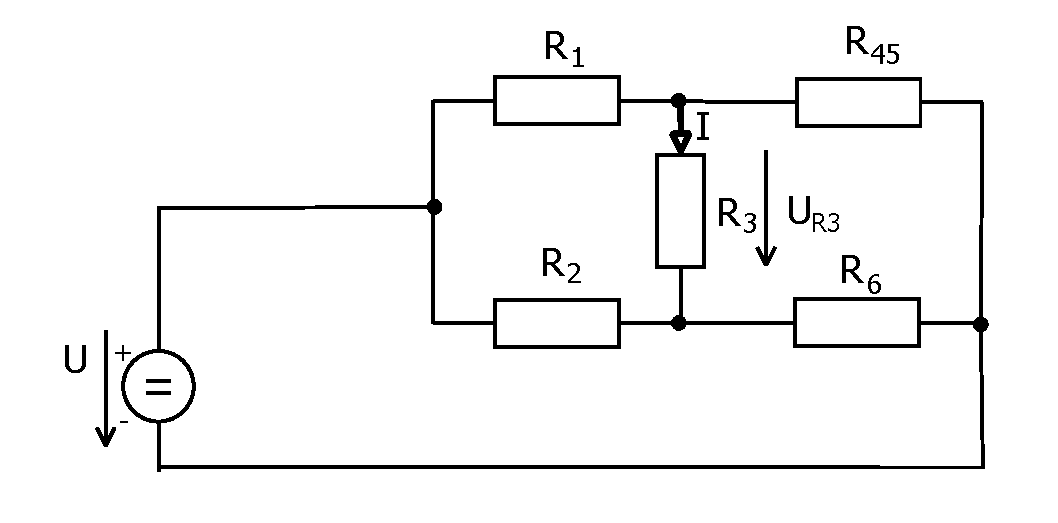
\includegraphics[width=0.6\linewidth]{obr/2_1.pdf}
		\caption{$R_4$ a $R_5$ si můžeme zapojit do série}
	\end{figure}
\begin{gather*}
R_{45} = R_4 + R_5 = 205 + 560 = 765\Omega \\
\end{gather*}


\begin{figure}[H]
		\center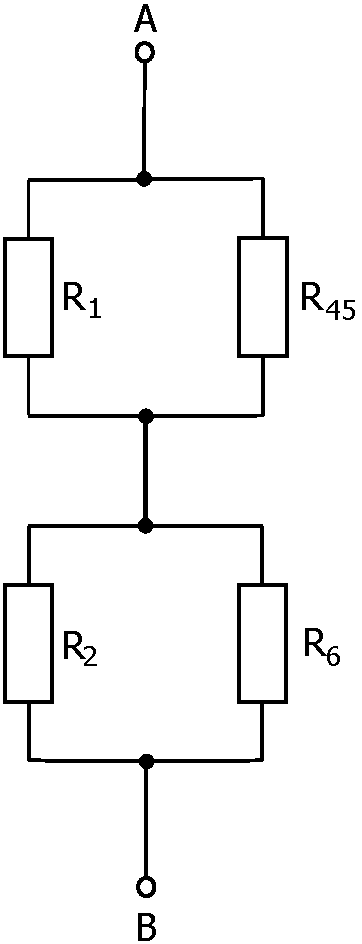
\includegraphics[width=0.25\linewidth]{obr/2_2.pdf}
		\caption{Uděláme zdroj nahrazený zkratem}
	\end{figure}
	
\begin{gather*}
R_I = \frac{R{1}\cdot R{45}}{R{1} + R{45}}+\frac{R{2}\cdot R{6}}{R{2} + R_{6}} = \frac{190\cdot 765}{190 + 765}+\frac{360\cdot 180}{360 + 180}\doteq 272.199 \Omega\
\end{gather*}

\begin{figure}[H]
		\center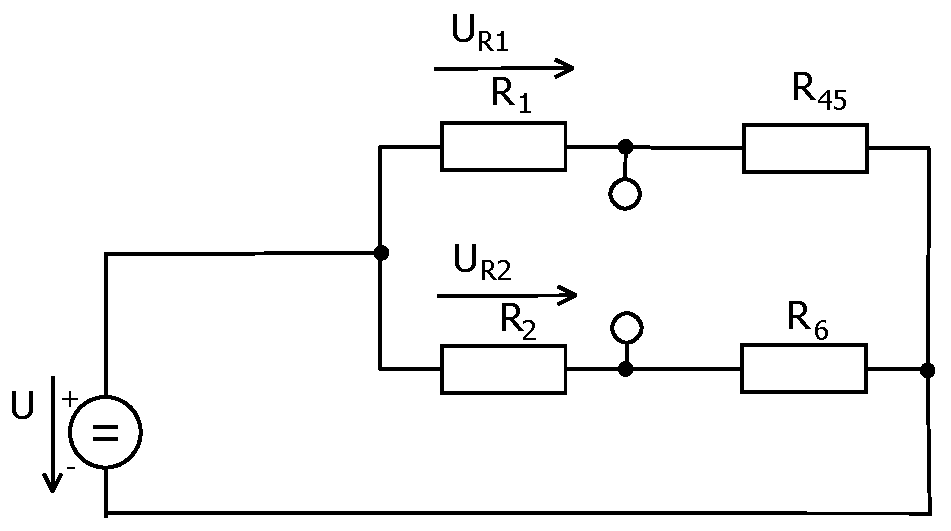
\includegraphics[width=0.6\linewidth]{obr/2_4.pdf}
		\caption{Obvod bez $R_3$}
	\end{figure}
	
\begin{gather*}
U_{R1}=\frac{R_1}{R_1+R_{45}}\cdot U_0=\frac{190}{190+765}\cdot 220\doteq43.76963V\\
U_{R2}=\frac{R_2}{R_2+R_6}\cdot U_0=\frac{360}{360+180}\cdot 220\doteq146.66667V\\
\end{gather*}

\begin{figure}[H]
		\center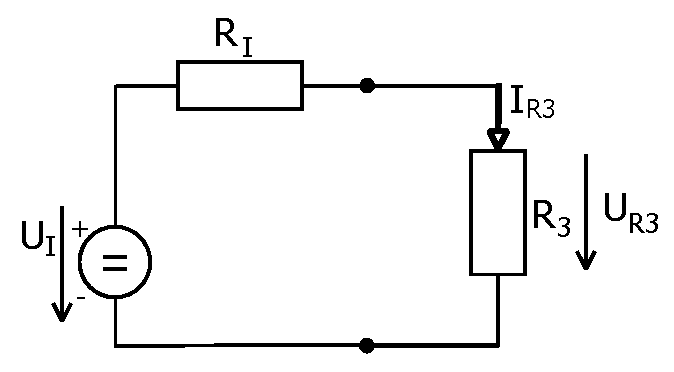
\includegraphics[width=0.6\linewidth]{obr/2_3.pdf}
		\caption{Schéma náhradního obvodu}
	\end{figure}
	
\begin{gather*}
U_i=U_{R2}-U_{R1}=146.66667-43.76963\doteq102.89704V\\
I_{R3}=\frac{U_i}{R_I+R_3}=\frac{102.89704}{272.199+580}\doteq0.1207A\\
U_{R3}=R_3\cdot I_{R3}=580\cdot0.1207\doteq70.006V
\end{gather*}